\chapter{The output mode cleaner}

\section{Motivation for an OMC}
The interferometer is supplied with a beam that has a very nearly pure Gaussian spatial profile thanks to the input mode cleaner. %NL%
The input mode cleaner is a nearly critically coupled resonant optical cavity which filters the beam supplied by the laser before it is delivered to the interferometer input. %NL%
The interferometer builds up power in the recycling cavity which is delivered to the long arms. %NL%
The arms further recycle the laser light and this large resonant field acts as the source field which gets modulated by a passing gravitational wave and pumps light into the audio sidebands which are finally detected as a signal. %NL%
Although the beam delivered by the mode cleaner is spatially very pure, the efficiency of coupling this beam to the final resonant mode of the arm is not ideal. %NL%
Components of the input light which are not matched to the mode of the arm cavity will not resonate and some of this unmatched light will exit the antisymmetric port along with the signal light. %NL%
The unmatched light at the antisymmetric port will exist as higher order modes (HOM) relative to the arm cavity mode and is often referred to as ``junk light.'' %NL%
The presence of this light on a photodetector will contribute photon shot noise. %NL%
Also, if the coupling is time dependent, the time variation of the junk light directly contaminate the signal with noise.

It is therefore desireable to be able to separate the junk light from the signal rich audio frequency fields originating in the arm cavities. %NL%
A natural form of spatial filter exists in the form of a critically coupled resonant optical cavity. %NL%
When placed at the output of the interferometer we refer to such a cavity as the output mode cleaner (OMC).

\infobox{The benefits of an OMC}{
\begin{itemize}
\item Reduce shot noise from HOM carrier fields
\item Reduce shot noise from RF sidebands
\item Reduce audio frequency noise from RF sidebands
\end{itemize}
}
It can be useful to point out that interferometers based on both RF and DC readout can benefit from an OMC \com{readouts discussed in previous chapter}. %NL%
Both the GEO and Virgo interferometers have used OMCs in an RF readout configuration, and LIGO experimented with an OMC before using DC readout \com{cite some things}. %NL%
An OMC is especially important for a DC readout interferometer because any audio frequency modulation of fields that are not the local oscillator or signal will contaminate the readout. %NL%
Also, there is not benefit of the frequency selection of the RF readout to selectively omit unwanted audio modulation. %NL%
An OMC may also be used to ensure the light provided by the differential arm offset dominates the DC power present on the detection photodiode, otherwise DC power from other fields (such as the RF sidebands) will contribute to photon shot noise without increasing the signal strength. %NL%


Thus, for an interferometer which employs DC readout, the OMC should efficiently strip the HOM field components of the carrier field as well as the RF sidebands. %NL%
This is achieved by creating a high finesse cavity that is controlled to resonate on the desired (carrier) field. %NL%
Ideally, being a critically coupled optical cavity, light incident on the OMC is totally transmitted on resonance. %NL%
The transmission of the off-resonant fields is goverened by the cavity finesse $\mathcal{F}$, explicitly the normalized transmission is
\begin{equation}
\label{eqn:finesse}
T=\frac{1}{1+\frac{4}{\pi^2}\mathcal{F}^2\sin{}^2\phi},
\end{equation}
where $\mathcal{F}$ is known as the \emph{cavity finesse} and $\phi$ is the detuning from resonance. %NL%
In terms of a frequency detuning of $\Delta f$ of the incident light, $\phi = \pi \Delta f / \mathrm{FSR}$.

\section{Optical and mechanical design of the OMC}
Prior to Enhanced LIGO, experiments we performed using a OMC borrowed from the GEO600 interferometer to investigate the difficulties in using an OMC with LIGO. %NL%
Noise introduced from jitter of the OMC input beam due to air currents and mechanical vibrations spoiled the sensitivity of the LIGO detector when the OMC was used. %NL%
This meant that one of the most obvious lessons learned from these investigations was the need to house the OMC in a low vibration environment. %NL%
For Enhanced LIGO, it was decided that the OMC would be housed inside the vacuum system and would be isolated from vibrations of the environment through the use of a seismically isolated optics table as well as a suspension system to provide passive filtering of vibrations.

\subsection{Cavity optics}
The design of the OMC was chosen to be a four mirror bowtie cavity \com{cite something}. %NL%
This choice was made over that of a two mirror linear cavity so that there was spatial separation of the reflected beam. %NL%
An even number of mirrors was chosen such that the horizontal and vertical HOMs would experience the same overall phase shift and thus experience nearly the same frequency offset from resonance, reducing the chances of an accidental HOM resonance.

\begin{figure}
  \begin{center}
  \leavevmode
  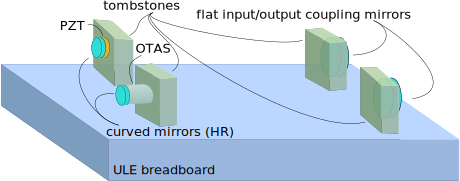
\includegraphics{figs-omc/construction.pdf}
  \end{center}
  \caption[Diagram of OMC cavity components]{Diagram of OMC cavity components. Auxilliary optics and sensors are not shown. The tombstones have holes (not pictured) machined in them to allow the laser beam to pass through.}
  \label{fig:omcconstruction}
\end{figure}

A diagram of the OMC may be seen in Figure \ref{fig:omcconstruction}. %NL%
The OMC optics are bonded with Vacseal expoxy onto custom designed fused silica optics mounts, called tombstones. %NL%
The tombstones were then bonded to a slab of Corning ULE Glass\footnote{The dimensions of the OMC breadboard are 450mm$\times$150mm$\times$39mm}, which we will refer to as the \emph{OMC breadboard}. %NL%
This arrangement fixed the cavity length to the desired value and was designed to be stable agains thermal variation. %NL%
The microscopic cavity length was controlled using a pair of actuators. %NL%
A fast PZT between one of the optics and its tombstone acted as a low range (1/10 FSR) high bandwidth (5kHz) length actuator. %NL%
Long range (several FSR) actuation was provided by one cavity mirror situated at the end of an aluminum tube heated by a ceramic heating element, affectionately reffered to as the OTAS.\footnote{OMC Thermal Actuation System}

A mode cleaner cavity is puporsefully designed such that HOMs do not ocuppy a degenerate resonance with the resonant \TEM{00} mode. %NL%
Cavities are commonly characterized by their stability $g$-parameter.\footnote{Asymmetric cavities are often given two $g$-parameters, one for each mirror (labeled 1 and 2) and $g=\sqrt{g_1 g_2}$.} The Gouy shift accumulated in the cavity is determined by the cavity geometry as \com{citation}
\begin{equation}
\label{eqn:gouyg}
\cos(\eta)=g
\end{equation}
where the $g$-parameter is usually given by $g=1-L/R$ for a linear cavity of length $L$ and mirror radius of curvature $R$. %NL%
The OMC is not a linear cavity, and it travels the length of the cavity only once during a full round trip. %NL%
To avoid confusion we will use the \emph{perimeter}, $p$, to denote the full round trip length. %NL%
One may substitute $2L=p$ in most formulae for linear cavities. %NL%
An extensive analysis was done by \com{Waldman} to determine the optimal cavity geometry to minimize the transmission of off-resonant HOM and frequency components trhough the OMC.\com{cite some waldman thing} The final design of the OMC was chosen to have a perimeter length of 1.042m, with 2m radius of curvature curved optics. %NL%
This gives a $g$-parameter of 0.7395 and a Gouy phase shift of $0.235\pi$ radians. %NL%
This implies that the fourth-order HOMs will accumulate almost $\pi$ radians relative to the \TEM{00} mode and be somewhat close to resonance.

\subsection{Sensors and auxilliary optics}
The gravitational wave signal readout is derived from the OMC trasmitted power. %NL%
The light trasmitted by the OMC is split by a near 50/50 beam splitter and detected on two photodiodes. %NL%
Both the beam splitter and photodiodes are located on the OMC breadboard. %NL%
The beamsplitter is glued to a tombstone similar to that of the cavity optics. %NL%
The photodiodes were attached to tombstones via a sandwich of metal plates screwed together around the tombstone. %NL%
This arrangement ensured that the OMC transmitted beam would not drift relative to the readout detectors.

A steering mirror on the OMC breadboard transmitted a small sample of the incoming beam allowing the input pointing to be analyzed by two quadrant photodetectors (QPDs). %NL%
A 50/50 beam splitter ditributed equal amounts of the input beam to the two QPDs. %NL%
The QPDs were located at different distances from the beam splitter to allow both beam angle and lateral position to be measured.

\subsection{Suspension system}
The OMC breadboard was suspended from a two stage vibration isolation suspension. %NL%
On the optics table was a large \com{steel} frame which housed the OMC. %NL%
A intermediate mass stage was suspended from the frame by two pendulum wires attached to the ends of blade springs. %NL%
The OMC breadboard was then suspended by four more wires attached to blade springs from the intermediate mass stage. %NL%
Servo control provided feedback damping of the suspension eigenmodes. %NL%
All actuation and sensing was performed on the intermediate stage, with actuation provided by electromagnetic coil actuators attached to the cage which applied forces to permanent magnets attached to the intermediate mass. %NL%
The actuator module also housed the sensing system which consisted of LED shadow sensors which measured the position of protruding flags attached to the magnets used for actuation.

\subsection{Mode matching telescope}
The beam exiting the interferometer from the antisymmetric port was directed through a beam steering and mode matching telescope. %NL%
The purpose of such a telescope is to correctly align and focus the beam exiting the interferometer to maximize the transmission of the gravitational wave signal through the OMC.

The steering optics were housed in a single pendulum suspension system. %NL%
The suspension and optics were collectively refered to as \emph{Tip-Tilt optics}. %NL%
The mounting and suspension of the beam steering optics underwent several modifications during the Enhanced LIGO project (see Chapter \ref{ch:jitter}). %NL%
The final configuration consisted of three highly reflective curved mirrors. %NL%
Two suspended by a single pendulum stage, with vertical isolation provided by blade springs, and a coil-magnet/shadow sensor system similar to that used in the OMC suspension. %NL%
The actuator system allowed feedback control of the optic angle for active beam alignment. %NL%
The third was housed in a similar suspension system, but without any sensing or actuation capabilities.

\subsection{Vibration isolation table}
The Tip-Tilts and OMC suspension frame were all housed in a single vacuum chamber and situated on top of a actively controlled seismic isolation table, the HAM-ISI.\footnote{HAM chamber Internal Seimic Isolation system} The HAM-ISI employed a single stage of passive vibration isolation, coupled with active feedback control using inertial sensors as the primary error signal. %NL%
A thorough account of the HAM-ISI design and performance can be found \com{Jeff's thesis?}.

\section{Characterization of the H1 OMC}
\begin{figure}
  \begin{center}
  \leavevmode
  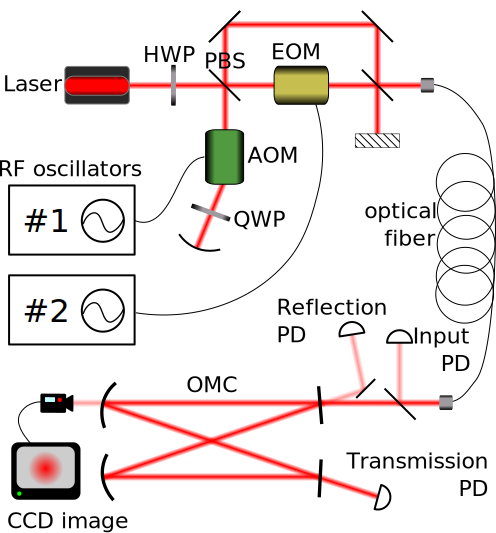
\includegraphics{figs-omc/interrogator.pdf}
  \end{center}
  \caption[Block diagram of OMC characterization setup.]{Block diagram of OMC characterization setup, also known as the OMC interrogator. The setup provides single mode laser light with RF sidebands for reflection locking, as well as a subcarrier with a tunable frequency.}
  \label{fig:interrogator}
\end{figure}

Figure \ref{fig:interrogator} shows a diagram of the experimental setup used to measure several parameters of the OMC which was installed on the H1 LIGO interferometer in Hanford, WA. %NL%
The laser source is a NdYAG NPRO providing a 1064nm wavelength laser beam. %NL%
The polarization is rotated by a half-wave plate (QWP). %NL%
A polarizing beam splitter (PBS) sends some fraction of the light through an electro-optic modulator (EOM) which is driven at by RF oscillator \#2. %NL%
The fraction transmitted by the PBS is tuned by changing the angle of the HWP. %NL%
The EOM introduces two RF sidebands which will be used for cavity length control. %NL%
The other path of light is director to an acouso-optic modulator (AOM). %NL%
The light is double passed though the AOM and and receives a frequency shift which is twice the frequency of RF oscillator \#1. %NL%
A quarter-wave plate (QWP) causes the polarization to rotate 90\degree{} after double passing, causing both paths to now be in the same polarization. %NL%
The light from the two paths are recombined before being injected into an optical fiber. %NL%
The frequency makeup of the combined beam includes the original carrier frequency, two RF sidebands and a frequency shifted subcarrier.

The light exiting the other end of the optical fiber is incident on the input coupling mirror of the OMC cavity. %NL%
A small sample of the input beam is incident on a photodetector. %NL%
The promptly reflected beam is detected on a photodetector where the photocurrent is demodulated at the frequency of RF oscillator \#2. %NL%
The frequency of oscillator \#2 is chosen so that it is outisde of the OMC resonance when the carrier is in resonancne. %NL%
This provides an error signal which is fed back to the frequency actuator of the laser. %NL%
The control system is able to maintain resonance of the laser in the OMC. %NL%
The laser transmitted through the OMC is detected on another photodetector. %NL%
A very small sample of the light in the cavity is transmitted through one of the HR mirrors and detected by a CCD sensor.

\subsection{Free spectral range}
Resonance occurs in the cavity when the total round trip phase of the incident laser beam as it propagates thorugh the cavity is an integer multiple of $2\pi$. %NL%
In terms of the frequency of the laser beam, this occurs at multiples of what is called the \emph{free spectral range} (FSR). %NL%
The FSR is related to the round trip cavity perimeter $p$ by $\mathrm{FSR}=c/p$.

The technique used to measure the cavity FSR involved locking the laser frequency so the carrier was resonant in the OMC while varying the frequency of the subcarrier and measuring the OMC transmitted power. %NL%
The OMC trasnmitted power will be maximized when the subcarrier is seperated from the carrier by a multiple of the FSR.

The RF freqeuncy generator was tuned to maximize the subcarrier transmission. %NL%
The error was just estimated by the smallest frequency step which did not cause a noticible change in transmission. %NL%
The measured FSR is
\begin{equation}
\mathrm{FSR}=278.288\pm0.001\text{MHz}.
\end{equation}
This corresponds to a cavity perimeter of 1.077m.

\subsection{Higher order mode spacing}
Similarly, the higher order mode frequency shift is measured by varying the subcarrier frequency until the subcarrier is resonant on a higher order mode of the OMC. %NL%
Coupling of the subcarrier beam into the HOMs is enhanced if slight misalignments are introduced on the input beam. %NL%
The identity of the higher order mode is determined by the image recorded by the CCD camera.

The HOM field components experience an effective frequency shift relative to the \TEM{00} carrier field due to the Gouy phase shift. %NL%
The effective frequency shift is given by
\begin{equation}
\label{eqn:gouyshift}
(m+n)\eta=\pi\frac{\Delta f}{\mathrm{FSR}}\mod \pi
\end{equation}
where $m$ and $n$ are the \TEM{mn} mode indicies, $\Delta f$ is the frequency shift, and $\eta$ is the Gouy phase shift. %NL%


Table \ref{tab:HOM} shows the measurements for several higher order mode frequency shifts. %NL%
Notice that the horizontal and vertical modes experience slightly different Gouy shifts in the cavity. %NL%
This is due to the astigmatism introduced in the cavity by non-normal incidence on the cavity mirrors. %NL%
One may use the measured $g$-parameters to estimate the radius of curvature of the curved optics of the OMC. %NL%
If we take the average value of the measured $g$s, this implies a radius of curvature of 1.96m, which is close to the specification of 2m.

\begin{table}
  \begin{center}
    \begin{tabular}{lll|ll}
      \hline
      $m$ & $n$ & $\Delta f$ & $\eta$ & $g$ \\
      \hline
      0 & 1 & -489.60 MHz & 0.2407$\pi$ & 0.7275\\
      1 & 0 & -489.12 MHz & 0.2424$\pi$ & 0.7238\\
      0 & 4 &  267.96 MHz & 0.2407$\pi$ & 0.7274\\
      4 & 0 &  269.60 MHz & 0.2422$\pi$ & 0.7242\\
      \hline
    \end{tabular}
  \caption[Higher order mode frequency shifts in the OMC]{Higher order mode frequency shifts in the OMC. The frequency shift measured by varying the subcarrier separation from the resonating carrier. The $m$ index is the horizontal mode order. Negative frequency shifts were acheived by using the -1 diffraction order of the AOM.}
  \label{tab:HOM}
  \end{center}
\end{table}

These data were taken with the OMC at room temperature. %NL%
It was discovered that the HOM spacing varied with the temperature of the thermal length actuator. %NL%
\com{Talk more about this? %NL%
it's own short section?}
\com{data here.}

\subsection{Cavity finesse}
The frequency profile of the transmitted peak when the subcarrier is shifted through resonance may be used to determine the cavity Finesse. %NL%
In the experiment, a sawtooth wave was used to sweep the subcarrier offset frequency while the OMC transmission was monitored. %NL%
These signals were digitized and recorded. %NL%
The recorded transmission versus frequency shift data are shown in Figure \ref{fig:finesseFit}. %NL%
The curve fit model used was Equation \ref{eqn:finesse} with $\phi=\pi \Delta f/\mathrm{FSR}$ and an arbitrary scaling and offset. %NL%
The fitting parameters return a cavity finesse of $367\pm2$.
\begin{figure}
  \begin{center}
  \leavevmode
  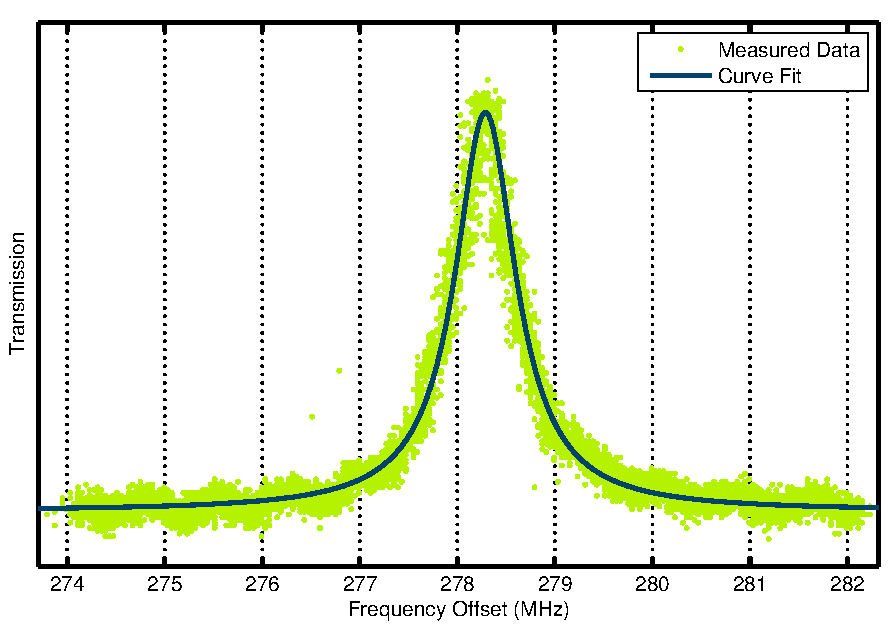
\includegraphics{figs-omc/finesseFit.pdf}
  \end{center}
  \caption[Measurement of the OMC transmission profile.]{Measurement of the OMC transmission profile. Subcarrier transmission while varying frequency offset. The width of the transmission peak is used to determine the cavity finesse. Fitted parameters give a finesse of $367\pm2$.}
  \label{fig:finesseFit}
\end{figure}

\subsection{Cavity losses}
The intra-cavity loss of the OMC was infered by using 3 photodetectors. %NL%
One measuring a sample of the input light, one measuring the reflected light, and one measuring the transmitted light. %NL%
Both the reflection and transmission photodiodes were calibrated relative to the input diode. %NL%
\com{figure showing calibration and measurement.} The calibration of the reflection diode was acheived by leaving the input and reflection diodes in place and blocking the beam inside the cavity. %NL%
The relative power readings of the diodes were then recorded and the ratio gives the reflection calibration. %NL%
One must also take into account the known transmission of the OMC input coupling mirror. %NL%
This calibration is done without moving the beam to be used during the measurement and mitigates systematic errors due to variations in the sensitivity of the surface of the diodes. %NL%
The trasnmission diode, however needed to be moved during calibration to measure the power incident on the cavity. %NL%
The trasnmission diode was also calibrated relative to the input diode.

This technique measures the light incident on the cavity, reflected from the cavity, and transmitted by the cavity. %NL%
Any light which is missing is assumed to be absorbed and constitutes cavity losses. %NL%
Table \ref{tab:lossmeas} shows the data taken to determine the cavity losses. %NL%
\com{what is the calculation} The cavity transmission was measured to be approximately 96\perc{}.

\begin{table}
  \begin{center}
    \begin{tabular}{lll|l}
      \hline
      Input (V) & Reflection (V) & Transmission (V) & Transmission Efficiency \\
      \hline
      0.95 & 1.51 & 0.53 & 0.965 \\
      0.903 & 1.44 &0.498 & 0.958\\
      \hline
    \end{tabular}
  \caption[Measurements of the OMC intra-cavity losses.]{Measurements of the OMC intra-cavity losses. All units are calibrated in Volts measured by the input PD.}
  \label{tab:lossmeas}
  \end{center}
\end{table}


\com{talk about degredation seen by squeezers}

\subsection{PZT actuator response}
The PZT length actuator of the OMC was calibrated using by using applying a voltage to the PZT to sweep the cavity through both carrier and subcarrier resonances. %NL%
The subcarrier frequency offset was chosen to be close to one FSR seperated from the carrier. %NL%
The separation was $1\mathrm{FSR}+3.8$MHz. %NL%
In terms of a change in cavity length, this is 14.5nm, which is twice the distance moved by the mirror. %NL%
Given the known frequency separation of the carrier and subcarrier, a determintation of the voltage offset between resonances can be used to calibrate the PZT. %NL%
The data taken are show in Figure \ref{fig:pztsweep}, and the mean offset of the central three ramps is 19.8V. %NL%
Thus the PZT calibration is $\frac{14.5\text{nm}}{2}\frac{1}{19.8\text{V}}=0.37\text{nm}/\text{V}$.
\begin{figure}
  \begin{center}
  \leavevmode
  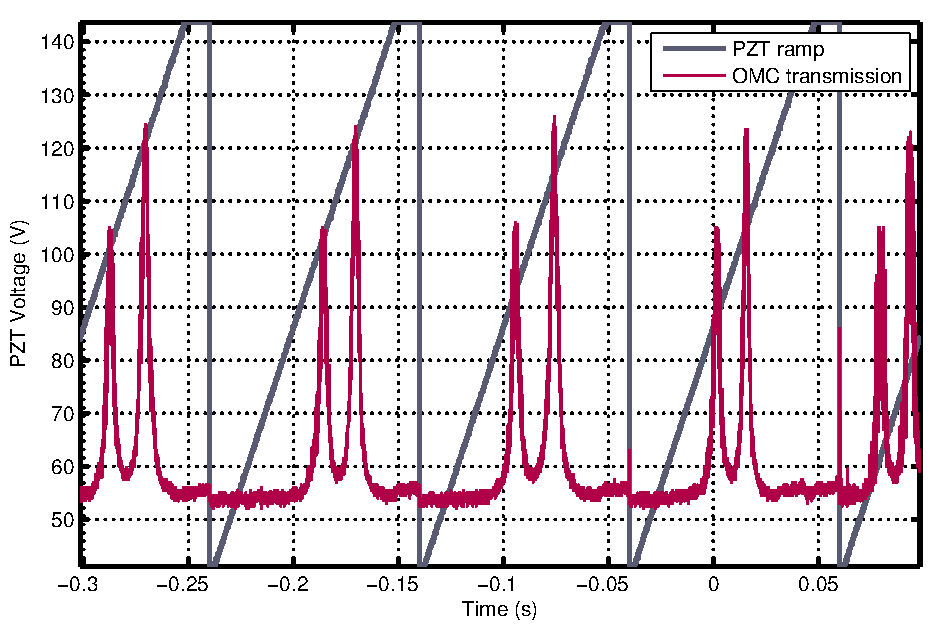
\includegraphics{figs-omc/pztdccal.pdf}
  \end{center}
  \caption[Measurement of the OMC PZT actuator calibration.]{Measurement of the OMC PZT actuator calibration. Both the carrier and subcarrier can be seen passing through resonance.}
  \label{fig:pztsweep}
\end{figure}

The high frequency response of the OMC PZT actuator was measured by locking the cavity on resonance for the carrier, and applying a periodic drive to the PZT. %NL%
The cavity locking error signal was used as a length response readout. %NL%
Figure \ref{fig:pzttf} shows the measured transfer function.

\begin{figure}
  \begin{center}
  \leavevmode
  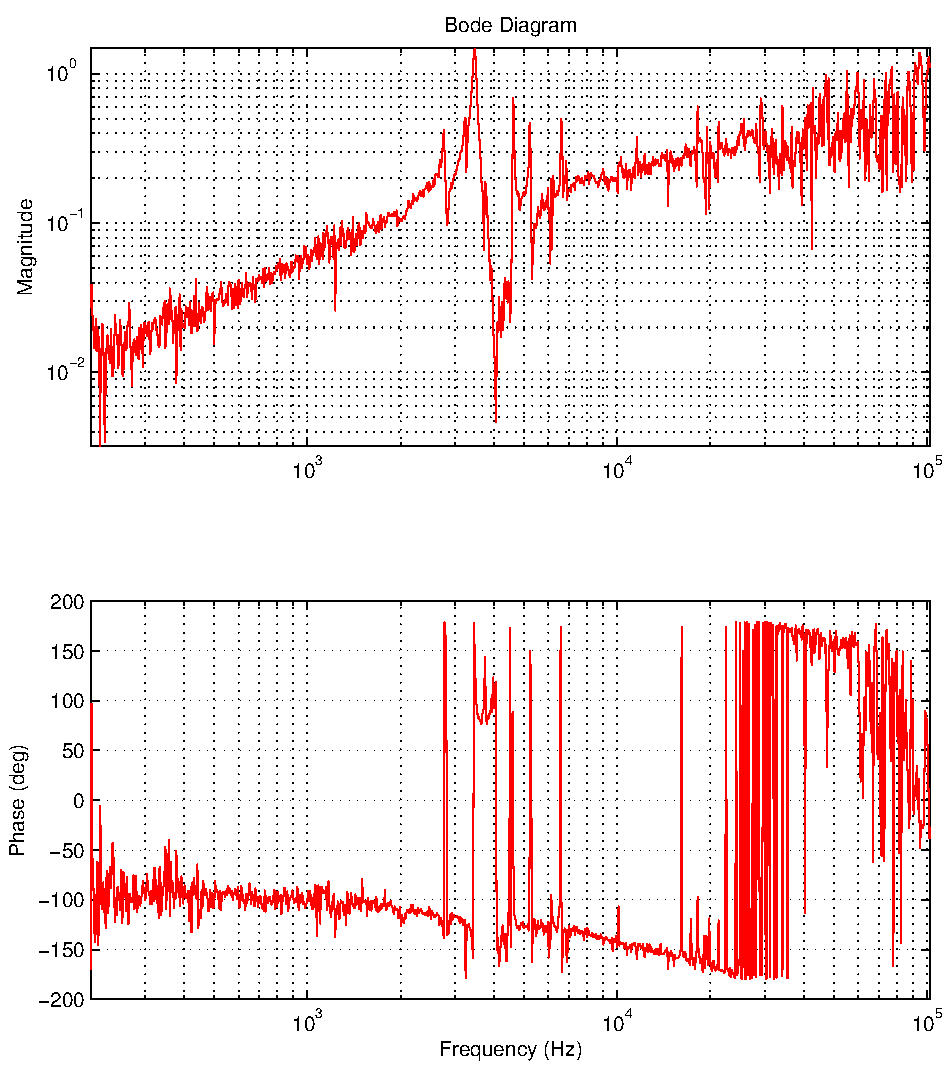
\includegraphics{figs-omc/pzttf.pdf}
  \end{center}
  \caption[Measurement of the OMC PZT actuator frequency response.]{Measurement of the OMC PZT actuator frequency response. \com{make a nicer figure}}
  \label{fig:pzttf}
\end{figure}


\section{Opto-thermal-mechanical feedback issues in the OMC}

\com{At least include measurements by Tim and I, hopefully can hack a model to explain it.}

%%% Local Variables: 
%%% mode: latex
%%% TeX-master: "main"
%%% End: 
